\section{Experimento 6 - Análisis de una señal modulada en frecuencia}
Para este experimento se utilizaron dos generadores de funciones conectados de la siguiente forma para obtener una señal modulada en frecuencia FM, en el caso de este experimento no se utilizó la resistencia de 1k$\Omega$ ya que el generador 2 poseía un atenuador incorporado.
\begin{figure}[H]
    \centering
    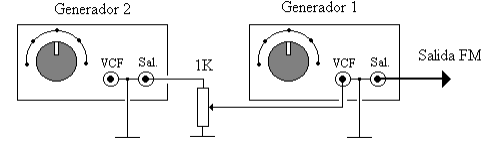
\includegraphics[width=0.5\textwidth]{images/experimento6.png}
    \caption{Diagrama de conexión del experimento 6.}
    \label{fig:experimento6}
\end{figure}

Una vez conectados los generadores de funciones con una salida de onda senoidal, el generador 1 se configuró a $50KHz$ con la perilla de amplitud a la mitad y el generador 2 a $1KHz$ con la perilla de amplitud a un cuarto. Luego se conecta el osciloscopio a la salida configurando la base de tiempos a $1ms/div$ y utilizando el modo FFT con la ventana en Hanning, Zoom X10 y en adquisición promedio de 64 cuentas.
\begin{figure}[H]
    \centering
    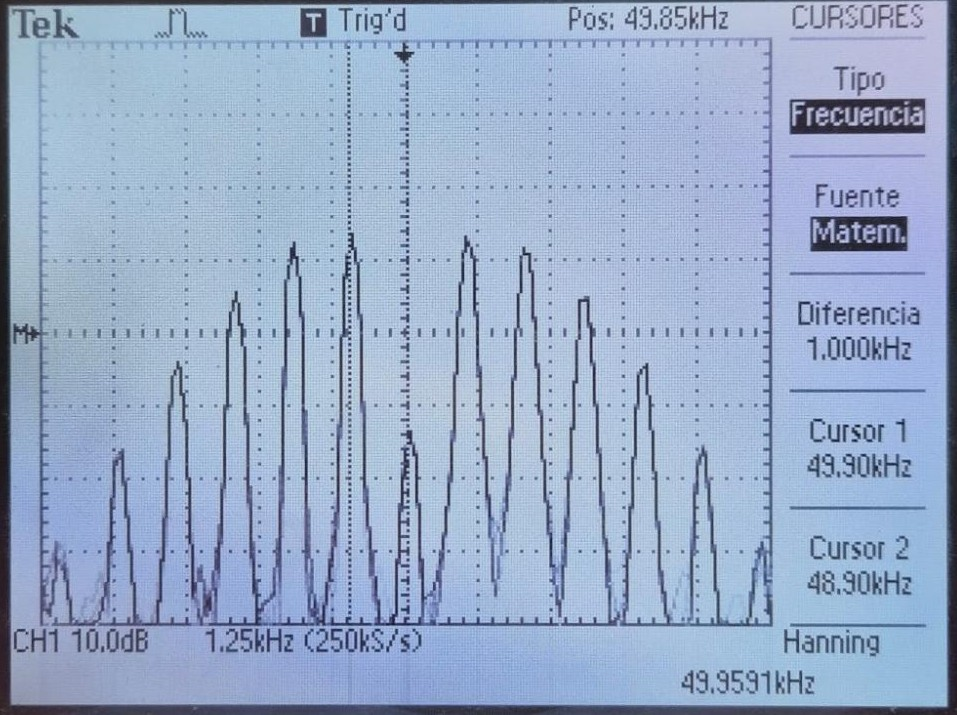
\includegraphics[width=0.5\textwidth]{images/exp6.jpg}
    \caption{FFT de la señal modulada en frecuencia.}
    \label{fig:experimento6_1}
\end{figure}


Luego de observar las diferencias de las presentaciones obtenidas variando el tipo de ventana se determinó que la ventana Hanning es la que mejor se ajusta a la señal modulada en frecuencia, ya que permite observar con mayor claridad los picos de la señal y así medir mejor las frecuencias de estos.
De esta forma se efectuaron las siguientes mediciones:
\begin{itemize}
    \item Frecuencia de la portadora: $49,9KHz$
    \item Frecuencia lateral superior e inferior: $48,9KHz$
    \item Frecuencia modulante(Diferencia): $1KHz$
\end{itemize}
